\documentclass{article}

\usepackage[final]{neurips_2019}

\usepackage[utf8]{inputenc}
\usepackage[T1]{fontenc}
\usepackage{hyperref}
\usepackage{url}
\usepackage{booktabs}
\usepackage{amsfonts}
\usepackage{nicefrac}
\usepackage{microtype}
\usepackage{graphicx}
\usepackage{xcolor}
\usepackage{lipsum}
\usepackage{subfig}
% \usepackage[nomarkers,nolists,figuresonly]{endfloat} %comment out when finish
\usepackage{amsmath}
\usepackage{booktabs}
\usepackage{multirow}
\usepackage{float}


\newcommand{\note}[1]{\textcolor{blue}{{#1}}}

\title{
  BERT Multitask Learning in a Semi-Supervised Learning Setup \\
  \vspace{1em}
  \small{\normalfont Stanford CS224N Default Project}  % Select one and delete the other
}

\author{
  Danhua Yan \\
  Department of Computer Science \\
  Stanford University \\
  \texttt{dhyan@stanford.edu} \\
  % Examples of more authors
%   \And
%   Name \\
%   Department of Computer Science \\
%   Stanford University \\
%   \texttt{name@stanford.edu} \\
%   \And
%   Name \\
%   Department of Computer Science \\
%   Stanford University \\
%   \texttt{name@stanford.edu}
}

\begin{document}

\maketitle

\begin{abstract}
Fine-tuning the BERT model for optimal performance across various NLP tasks necessitates 
high-quality labeled data, which can be challenging to obtain. Semi-supervised learning (SSL) 
utilizes unlabeled data to bolster supervised learning tasks. In this study, we enhance 
BERT\textsubscript{BASE} embeddings across multiple tasks, including fine-grained sentiment 
classification, paraphrase detection, and textual similarity, by implementing a multitask 
learning strategy. We employ a fused sentence embedding approach and a simultaneous training 
schedule to ensure balanced performance across tasks. Furthermore, we explore the effectiveness 
of Unsupervised Data Augmentation (UDA) in SSL settings, using various data augmentations 
generated by Pre-trained Language Models (PLMs). 
We also provide 
insights into the strengths, limitations, and ethical considerations of our model.
The culmination of our efforts resulted in an overall accuracy of 0.763 on the test dataset. 
Task-specific performances included a score of 0.517 on the SST5, 0.839 on the QQP, and 0.866 
on the STS dataset. These results signify a substantial improvement in multi-task learning 
capabilities.

% An abstract should concisely (less than 300 words) motivate the problem, describe your aims, describe your contribution, and highlight your main finding(s). 
\end{abstract}


\textbf{Key Information to include}
% \begin{itemize}
%     \item Mentor:
%     \item External Collaborators (if you have any):
%     \item Sharing project:
% \end{itemize}

TA Mentor: Kamyar John Salahi | No external collaborators or mentor | Not sharing projects

% {\color{red} This template does not contain the full instruction set for this assignment; please refer back to the milestone instructions PDF.}

\section{Introduction}
% The introduction explains the problem, why it's difficult, interesting, or important, 
% how and why current methods succeed/fail at the problem, and explains the key ideas of your approach and results. Though an introduction covers similar material as an abstract, the introduction gives more space for motivation, detail, references to existing work, and to capture the reader's interest.

BERT, an innovative NLP model developed by \cite{devlin2019bert}, utilizes transformer 
architecture and attention mechanisms to understand contextual word relationships. 
Recent studies have leveraged pre-trained BERT weights, fine-tuning the model to achieve 
outstanding results across a variety of tasks. However, acquiring labeled data 
for BERT fine-tuning can be challenging and often not feasible.

Semi-supervised learning (SSL) is a widely used technique that leverages unlabeled data 
to enhance the performance of supervised learning tasks. Among the various SSL methods, 
consistency training stands out for its proven effectiveness across numerous benchmarks. 
This method ensures that a model produces consistent outputs for an unlabeled example, 
even when subjected to minor perturbations, such as the introduction of small noise.
This approach sheds light on training high performance NLP models with limited labels.

In this study, we enhance the performance of BERT\textsubscript{BASE} embeddings 
across multiple tasks: fine-grained sentiment classification, paraphrase detection, 
and textual similarity. We introduce a multitask learning strategy that employs a 
fused sentence embedding approach for combining pairwise sentence inputs, and a
simultaneous training schedule is implemented to balance performance across tasks.
We also utilize the Unsupervised Data Augmentation (UDA) framework proposed by
\cite{xie2020unsupervised} in SSL 
settings, to further investigate the effectiveness of UDA with various data 
augmentations generated by Pre-trained Language Models (PLMs). 
Through experiments and thorough analyses, we offer
insights into the strengths, limitations, and ethical considerations of our model.

\section{Related Work}

BERT, along with its subsequent PLMs, has sparked extensive 
research aimed at enhancing their performance on out-of-domain downstream tasks. Fine-tuning 
pre-trained weights has become standard practice, and researchers are continually developing 
strategies and architectures to further improve BERT embeddings.

For downstream tasks like paraphrase detection and textual similarity, the quality of 
sentence pair embeddings is pivotal to the performance of the model. In the original 
BERT implementation, \cite{devlin2019bert} utilized a pair of sentences separated by 
the \texttt{[SEP]} token and performed next sentence prediction to enhance token 
embeddings. This method, due to the intrinsic context embeddings learned by BERT, has 
been widely adopted for tasks involving sentence pairs.
\cite{reimers2019sentencebert} introduced the Sentence-BERT architecture where, during 
training, each sentence is encoded by BERT separately, and the joint embedding is an 
absolute element-wise difference. At inference time, cosine similarity is computed 
directly between the two separate embeddings to calculate similarity scores.
\cite{choi2021eval} explored different pooling strategies beyond the \texttt{[CLS]} token 
representation in the SBERT setup, demonstrating that advanced CNN pooling can enhance 
textual similarity tasks. These studies underscore the significance of single sentence 
and sentence pair embeddings in the performance of the final models.
In this study, we investigate various encoding strategies and their influence on 
the multi-task learning performance.

% Related work about SSL enhancing the work (from UDA)
Fine-tuning for diverse downstream tasks can be challenging due to the limited availability 
and high acquisition cost of task or domain-specific labeled datasets. Despite this, 
deep learning systems typically require substantial data to function optimally. Semi-supervised 
Learning (SSL) emerges as a promising paradigm, leveraging a small labeled dataset in 
conjunction with a large unsupervised dataset to construct effective and generalizable 
NLP models. Consistency training, a subset of SSL, has demonstrated its efficacy across 
numerous benchmarks \cite{ctNIPS2014_66be31e4,ctrasmus2015semisupervised,ctlaine2017temporal,cttarvainen2018mean}.

The Unsupervised Data Augmentation (UDA) framework, proposed by \cite{xie2020unsupervised}, 
establishes a strong connection between data augmentation and semi-supervised learning,
that improved data augmentation techniques can significantly enhance semi-supervised learning 
outcomes. For NLP tasks, the study explored back-translation\footnote{This process involves 
translating a text from language $A$ to language $B$, and then back to $A$ to generate an 
augmented example.}, which demonstrated performance improvements when dealing with limited 
data labels.
The recent success of PLMs such as ChatGPT and LLaMA-3 
has empowered researchers to harness their robust knowledge retrieval capabilities. 
This has facilitated the generation of training datasets and data augmentations 
(\cite{zhong2022efficient, wang2021zerolabel, raffel2023exploring}), leading to 
remarkable performance on multi-task NLP benchmarks like GLUE \cite{wang2019glue} 
and SuperGLUE \cite{wang2019superglue}. Training samples are generated 
from few-shot or zero-shot prompts and combined with unlabeled datasets to 
fine-tune BERT-like models leveraging UDA-like framework 
(\cite{meng2022generating,wang2021zerolabel}).
In this study, we utilize the UDA framework to investigate efficient fine-tuning strategies for 
transitioning supervised learning into SSL settings, aiming to enhance the performance of 
supervised NLP tasks. We conduct experiments with advanced PLMs to generate data augmentations, 
examining whether this approach can yield high-quality data that strengthens SSL.


\section{Approach}
% This section details your approach(es) to the problem. 
% For example, this is where you describe the architecture of your neural network(s), and any other key methods or algorithms.

We adhere to the original BERT setup, using the pre-trained 
BERT\textsubscript{BASE} model weights for downstream tasks. We have fine-tuned the BERT 
embeddings through the implementation of various extensions, including those commonly 
used in SSL, to enhance their generalization capabilities 
across multiple tasks.

\subsection{Baseline} 
In our study, the multi-task baseline uses frozen pre-trained BERT\textsubscript{BASE} 
embeddings, learning only a single linear projection layer as task head. For handling
sentence-pair tasks, embeddings of the two sentences are concatenate to form
a joint representation of the sample before feeding into the task head.


\subsection{Combining Sentence Embeddings}
\label{sec:sent-pari-embed}
For sentence-pair NLP tasks,
we explored two categories of architectures for combining sentence embeddings, as illustrated 
in Figure \ref{fig:example}. The first architecture, Pooling Separate Embeddings, 
generates a joint embedding from two sentences encoded separately by BERT. We experimented 
with various methods, including simple concatenation (as used in the baseline), absolute 
difference (inspired by the SBERT framework training step \cite{reimers2019sentencebert}), 
direct cosine similarity with scaling, and dot product attention of the two embeddings, 
which employs an attention matrix to embed the sentence pair.
The second architecture, Fused Sentence Embedding, utilizes BERT's inherent training 
with sentence pairs separated by the \texttt{[SEP]} token to encode sentence context 
similarities. This approach combines the two sentences into a single input sequence to 
produce a unified embedding. 


\begin{figure}[h]%
  \centering
  \subfloat[\centering Archetecture 1: Pooling seperate embeddings]
  {{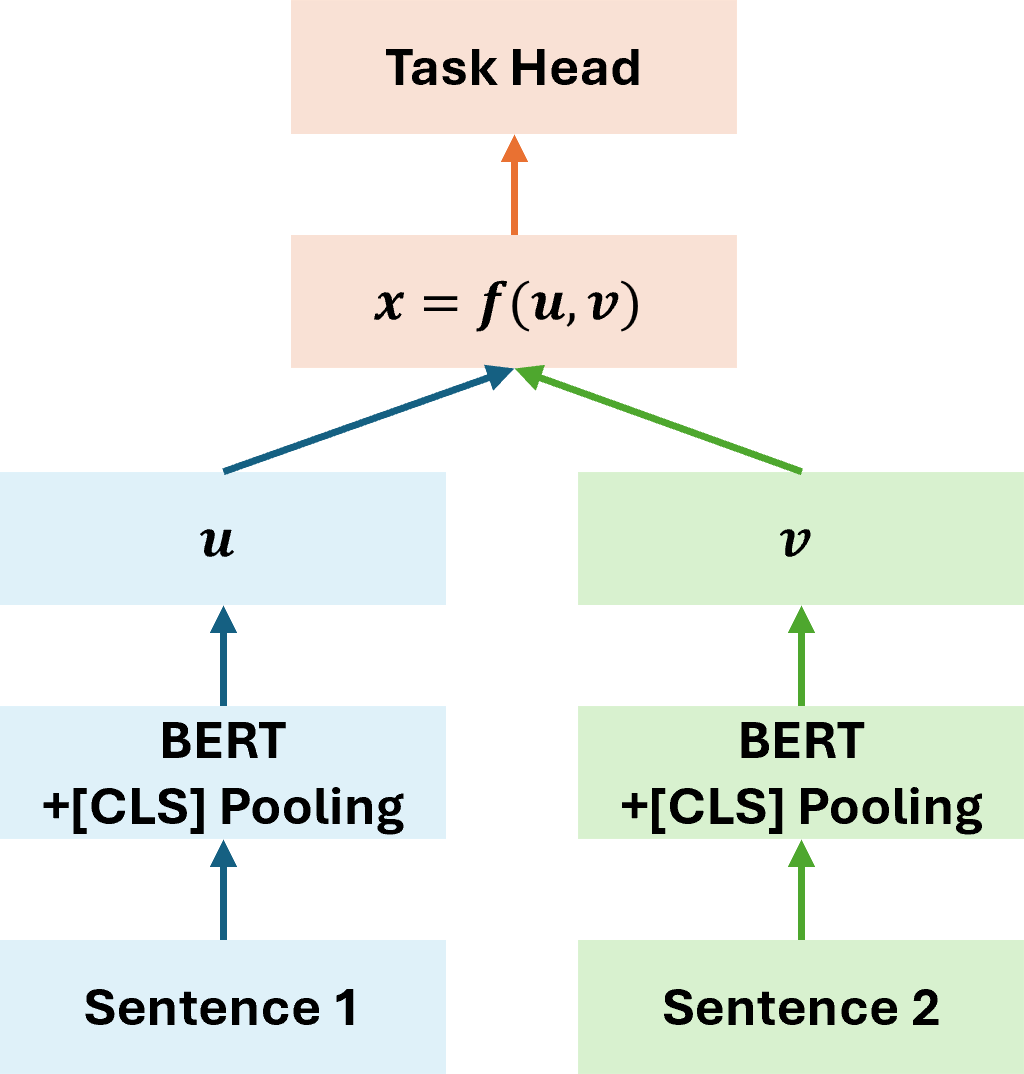
\includegraphics[height=3.5cm]{pics/combine_1.png} }}%
  \qquad
  \subfloat[\centering Archetecture 2: Fused sentence embedding]
  {{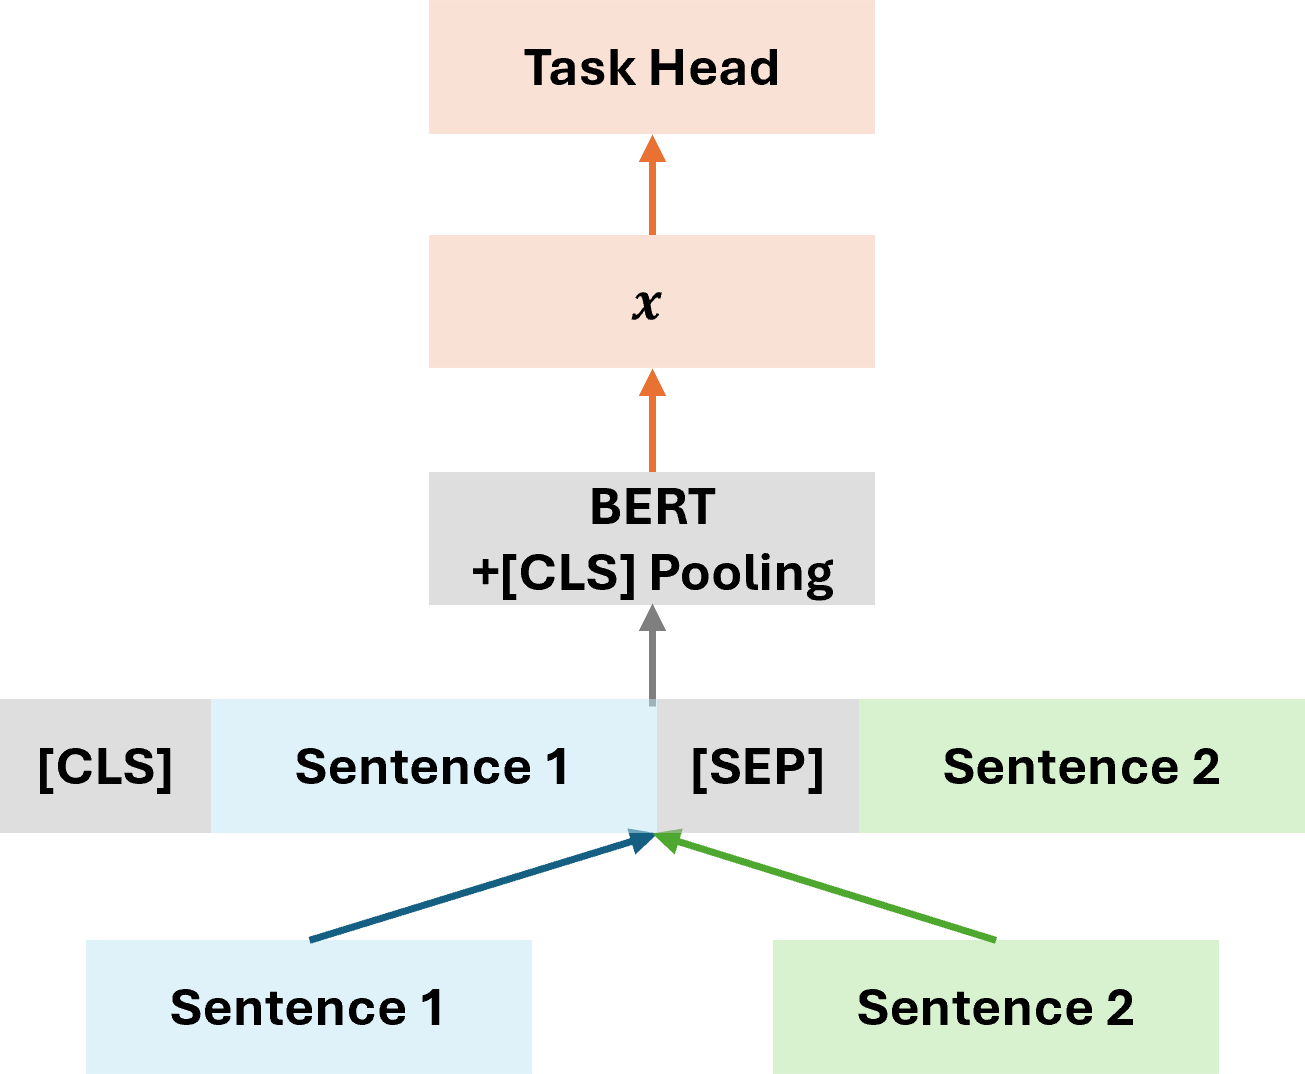
\includegraphics[height=3.5cm]{pics/combine_2.png} }}%
  \caption{Two architectures for sentence-pair inputs: 
  (a) Each sentence is BERT-encoded separately, then pooled into a single embedding.
  (b) Sentence-pairs are concatenated with a \texttt{[SEP]} token and BERT-encoded into 
  one embedding.
  }%
  \label{fig:example}%
\end{figure}

\subsection{Training Strategies}
To ensure the fine-tuned BERT embeddings generalize across all downstream tasks, we 
employ two training strategies. In Sequential Training, tasks are trained in succession 
within each epoch. Specifically, model weights are updated per batch, with three tasks 
forming a batch queue in the order of paraphrase detection, textual similarity, and 
sentiment analysis.
Conversely, Simultaneous Training aggregates the losses for all tasks concurrently. 
Each batch comprises three different tasks of the same batch size, and losses are 
summed without weighting.

\subsection{Semi-Supervised Learning Setup}
Motivated by the success of UDA (\cite{xie2020unsupervised}), we transform supervised tasks 
into semi-supervised ones to investigate effective fine-tuning strategies. 
We eliminate all labels from the training sets to create an unlabeled dataset and 
generate data augmentations of these examples by prompting advanced PLMs (e.g., ChatGPT or 
LLaMA-3) in various ways.
Despite the availability of open-source code accompanying the UDA paper, \textbf{we opted 
to implement this framework from scratch} to gain a deeper comprehension of each 
component's functionality.

\subsubsection{Advanced data augmentation}
\label{sec:appr_data_aug}
We explored three distinct text augmentation strategies. The first, back-translation, 
is proposed by the UDA authors. It involves prompting the PLM to translate a given 
English sentence into French, then back into English. This method maintains the 
original meaning and factuality of the sample, albeit with potential changes in 
word choice and phrasing.
The other two strategies, sentence completion and random-mask completion, are original 
approaches. Sentence completion involves providing the PLM with the sample sentence, 
appending \texttt{"To put it differently,"} at the end, and allowing the PLM to complete the 
sentence. This strategy aims to ensure the PLM comprehends the sentence's meaning and 
elaborates on its context.
Random-mask completion randomly masks consecutive words and prompts the PLM to fill 
in the masked blank using a roughly equivalent number of words. This strategy aims to 
create structurally similar text augmentations, albeit with the risk of altering the 
factuality of the sentence, even if it appears very similar.

\subsubsection{SSL Loss}
In a typical SSL setup, loss function is usually a combination of 
supervised loss $\mathcal{L}_{\text{sup}}$ and unsupervised loss $\mathcal{L}_{\text{unsup}}$.
Following UDA paper's setup, here $\mathcal{L}_{\text{sup}}$ is the mean cross-entropy loss,
and $\mathcal{L}_{\text{unsup}}$ is the mean KL-divergence loss between unsupervised and 
augmented data.
Formally, given labeled dataset $L$ and unlabeled dataset $U$, we aim to learn a 
classification model $p_{\theta}$ with parameters $\theta$. This model maps input $x$ to a 
class distribution $\hat y = p_{\theta}(x)$. We denote data augmentation as $q(\cdot)$, 
where $\hat x = q(x)$ is the augmented input. Our goal is to find $\theta$ minimizing the 
loss function $J(\theta) = \mathcal{L}_{\text{sup}} + \lambda \mathcal{L}_{\text{unsup}}$, 
and $\lambda$ is the 
regularization coefficient.

\subsubsection{Training Signal Annealing (TSA)}
To mitigate the risk of overfitting to labeled samples prematurely, we incorporate the 
TSA into the supervised loss. This approach, proposed 
by the UDA authors, dynamically selects a subset of the labeled dataset, $L_t$, at each 
training step $t$, defined as $L_t = \{x \in L \mid p_{\theta}(x) \leq 
\eta(t)\}$, where $\eta(\cdot)$ is a threshold function that sets a dynamic threshold at 
each step $t$. 
Here we test linear, log, and exponential $\eta(\cdot)$ and assess the effectiveness in
reducing overfitting.

\subsubsection{Confidence Masking on KL-divergence Loss}
To focus the unsupervised loss on distribution discrepancies arising from suboptimal data 
augmentation, we calculate the loss only on a subset of the unlabeled data where the model 
is confident in its prediction. Specifically, at step $t$, we compute the loss among $U_t$, 
where $U_t = \{x \in U \mid p_{\theta}(x) > \beta\}$, and $\beta$ is a constant confidence 
level. 

\subsubsection{Loss Function}
The final loss function used for this study combining all above becomes:
$$\mathcal{L} = 
- \mathbb{E} \left[ \sum_{i=1}^{|L_t|} y_i \log p_{\theta}(x_i) \right]
- \lambda \mathbb{E} \left[ \sum_{j=1}^{|U_t|} p_{\tilde{\theta}}(x_j) \log 
\frac{p_{\tilde{\theta}}(x_j)}{p_{\theta}(\hat x_j)} \right]
$$

Note that the term $\tilde{\theta}$ denotes a \textit{fixed} copy of the current parameters, 
to indicate that the gradient is not propagated through $\tilde{\theta}$.
This is to ensure the loss is minimizing the divergence against a stable reference against
current model parameters (\cite{miyato2018virtual}).

\section{Experiments}
% This section contains the following.

\subsection{Data}
% Describe the dataset(s) you are using (provide references). If it's not already clear, make sure the associated task is clearly described.
% Being precise about the exact form of the input and output can be very useful for readers attempting to understand your work, especially if you've defined your own task.
We fine-tuned the pre-trained BERT\textsubscript{BASE} model using three benchmark datasets 
from the default project: Quora Question Pairs (QQP), SemEval STS Benchmark (STS), and 
Stanford Sentiment Treebank (SST5). For each dataset, we utilized the \texttt{train} split. 
Specifically, for the QQP dataset, we consistently used a fixed subset of 14,057 training 
samples, representing 5\% of the provided training data, throughout our experiments.

We leveraged the same training datasets for unsupervised learning by omitting the provided labels. 
Data augmentation of these unsupervised datasets was achieved by prompting the LLaMA-3 Chat 
(8B) model via the TogetherAI API using various prompts.

\subsection{Evaluation method}
% Describe the evaluation metric(s) you use, plus any other details necessary to understand your evaluation.
% Some projects will have clear metrics from prior work on given datasets, but we realize that other projects will define their own metrics.
% If you're defining your own metrics, be clear as to what you're hoping to measure with each evaluation method (whether quantitative or qualitative, automatic or human-defined!), and how it's defined.
We evaluated our models using standard metrics pertinent to each task. 
For QQP and SST5, we use accuracy to assess the classification performance. 
For STS, we use the Pearson correlation of the true similarity values against the predicted 
similarity values.

\subsection{Experimental details}
% Report how you ran your experiments (e.g., model configurations, learning rate, training time, etc.)
All experiments used the BERT\textsubscript{BASE} model with pre-trained weights. The 
baseline model's task head projects BERT embeddings to target space using a linear layer, 
with SST5 and QQP tasks using softmax for predicted classes and cross entropy loss. STS 
task uses an amplified sigmoid layer for 0-5 regression output and MSE loss, and further
modified in SSL extension to a classification problem with 26 classes in 0.2 
increments. All models are trained using 
learning rate of 1e-5, and batch size of 8, and gradients are clipped at 0.1 to help
reduce potential noise from the SSL setup.
Unless otherwise noted,  models without TSA (i.e.
baseline and extension models) are trained 10 epochs, models in SSL settings are trained 50 epochs
with an early stopping patience of 10 epochs.
All models were trained using the AdamW optimizer, with $\beta_1 = 0.9, \beta_2 = 0.999$, 
and a weight decay regularization $\lambda = 0.01$.
For data augmentation generated by prompting LLaMA-3 Chat (8B) model via the TogetherAI API, 
we set request parameters as temperature = 0.5, repetition\_penalty = 1. 
For SSL loss, we follow UDA paper by choosing
unsupervised loss regularization $\lambda = 1$, confidence masking threshold $\beta = 0.8$,
and sharpen the unsupervised predictions using softmax temperature $\tau = 0.4$.
Experiments are performed on a Nvidia GeForce RTX 4070 Ti SUPER 16GB GPU.

% Please add the following required packages to your document preamble:
% \usepackage{booktabs}
\subsection{Baseline and Combining Sentence Embeddings}
\label{sec:baseline_ext}
Pre-trained BERT\textsubscript{BASE} embeddings struggle with complex tasks beyond binary 
classifications like SST5 and STS. Fine-tuning BERT on downstream tasks is necessary for 
optimal performance. In pursuit of the best sentence pair representation using approaches 
described in section \ref{sec:sent-pari-embed}, results in Table \ref{tab:baseline_ext} 
show that using intrinsic BERT \texttt{[SEP]} token significantly outperforms all other 
models across all tasks. BERT's next sentence prediction task enables embeddings to capture 
context similarity between two sentences more effectively. 
The absolute difference between embeddings captures 
sentence distance, performs reasonably well on the binary QQP task but falls short on 
nuanced STS tasks. 
Other methods may struggle due to an excess or deficiency of learned parameters, which may not 
align well with the sizes of the training data.

\begin{table}[H]
  \centering
  \caption{Comparisons of Baselines and Extensions on Dev Data, training three tasks simultaneously}
  \label{tab:baseline_ext}
  \begin{tabular}{@{}lcccc@{}}
    \toprule
    \textbf{Model}                & \multicolumn{1}{c}{\textbf{SST5}} & \multicolumn{1}{c}{\textbf{QQP}} & \multicolumn{1}{c}{\textbf{STS}} & \multicolumn{1}{c}{\textbf{\begin{tabular}[c]{@{}c@{}}Avg. Accuracy\end{tabular}}} \\ \midrule
    Baseline (last-layer only)    & 0.309                             & 0.667                            & 0.209                            & 0.527                                                                                 \\
    Arc1-Simple Concat            & 0.479                             & 0.738                            & 0.369                            & 0.634                                                                                 \\
    Arc1-Absolute difference      & 0.510                             & 0.733                            & 0.532                            & 0.670                                                                                 \\
    Arc1-Cosine Similarity        & 0.482                             & 0.533                            & 0.436                            & 0.578                                                                                 \\
    Arc1-Dot Product Attention    & \textbf{0.514}                    & 0.737                            & 0.486                            & 0.665                                                                                 \\
    Arc2-Fused Sentence Embedding & 0.501                             & \textbf{0.829}                   & \textbf{0.852}                   & \textbf{0.752}                                                                        \\ \bottomrule
    \end{tabular}
\end{table}

\subsection{Training Strategies}
Simultaneous training consistently surpasses sequential training in generating multitask models, 
and will be employed for the remainder of this study. For further details, refer to Appendix 
\ref{sec:appdx_train_strategy}.

\subsection{Semi-Supervised Learning Setup}
First, we evaluate the performance difference when changing the STS task from regression 
to a classification problem. In the single-dataset BERT 
fine-tuning experiment, the regression approach achieves a dev Pearson correlation of 0.868, 
while classification reaches 0.864. Given the marginal difference, we convert the STS model 
to classification to apply the same UDA framework on the STS dataset.

\subsubsection{Training Signal Annealing (TSA)}
Different threshold functions dictate the rate at which training signals of labeled 
examples are released. The exponential schedule predominantly releases signals towards 
the end of training, while the log schedule does the converse. As shown in Figure 
\ref{fig:tsa}, the TSA component proves effectiveness in mitigating overfitting during 
early epochs, thereby enhancing the overall model accuracy.
The Log schedule, which releases most training samples early, is less effective in 
curbing overfitting and performs comparably to the absence of TSA. Conversely, the 
Exponential schedule effectively mitigates overfitting, but requires a considerably 
longer duration to achieve comparable performance when training samples are plentiful.
The Linear schedule strikes a balance between convergence speed and the ability to 
prevent overfitting within 10 epochs, making it the chosen method for subsequent extensions.

\begin{figure}[H]%
  \centering
  \subfloat
  {{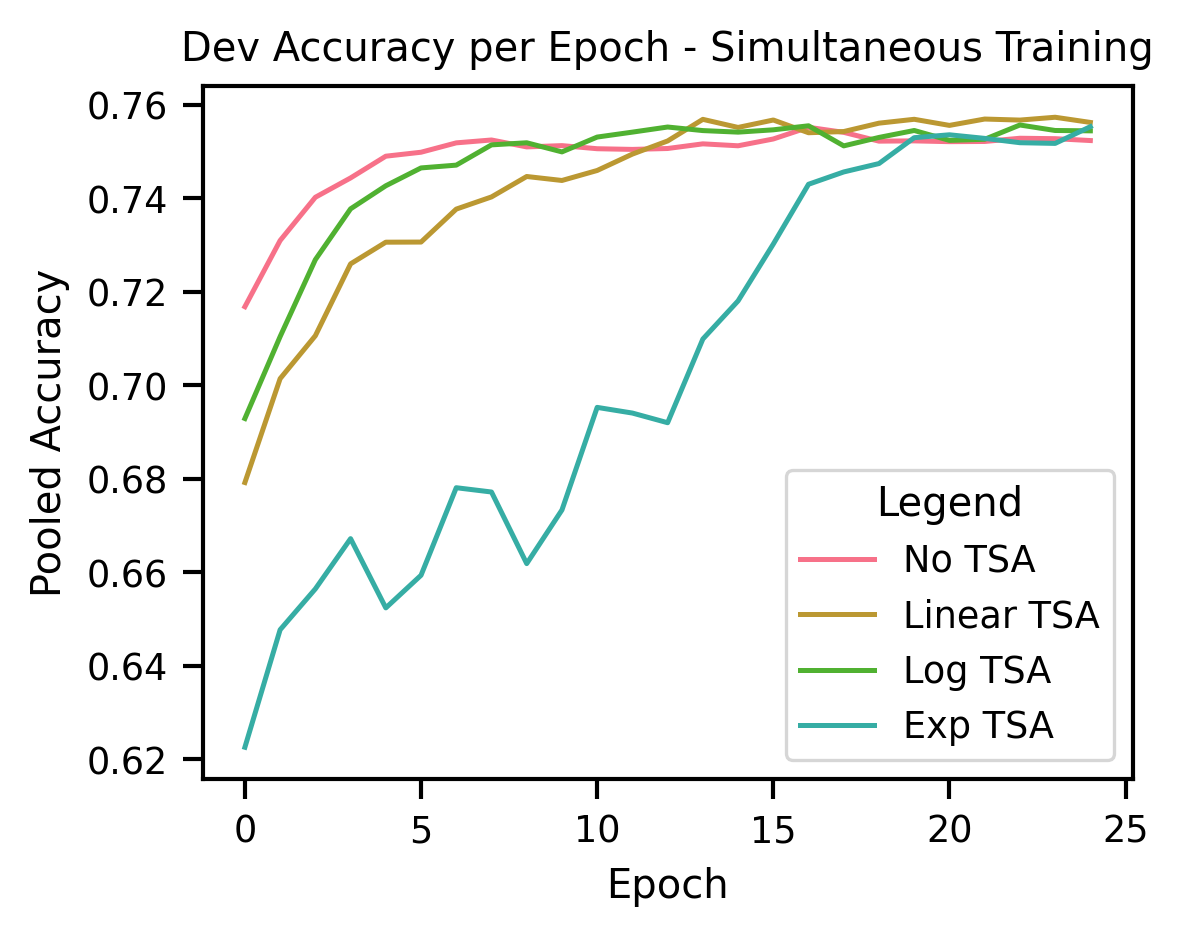
\includegraphics[height=5cm]{pics/tsa-simul-dev.png} }}%
  \qquad
  \subfloat
  {{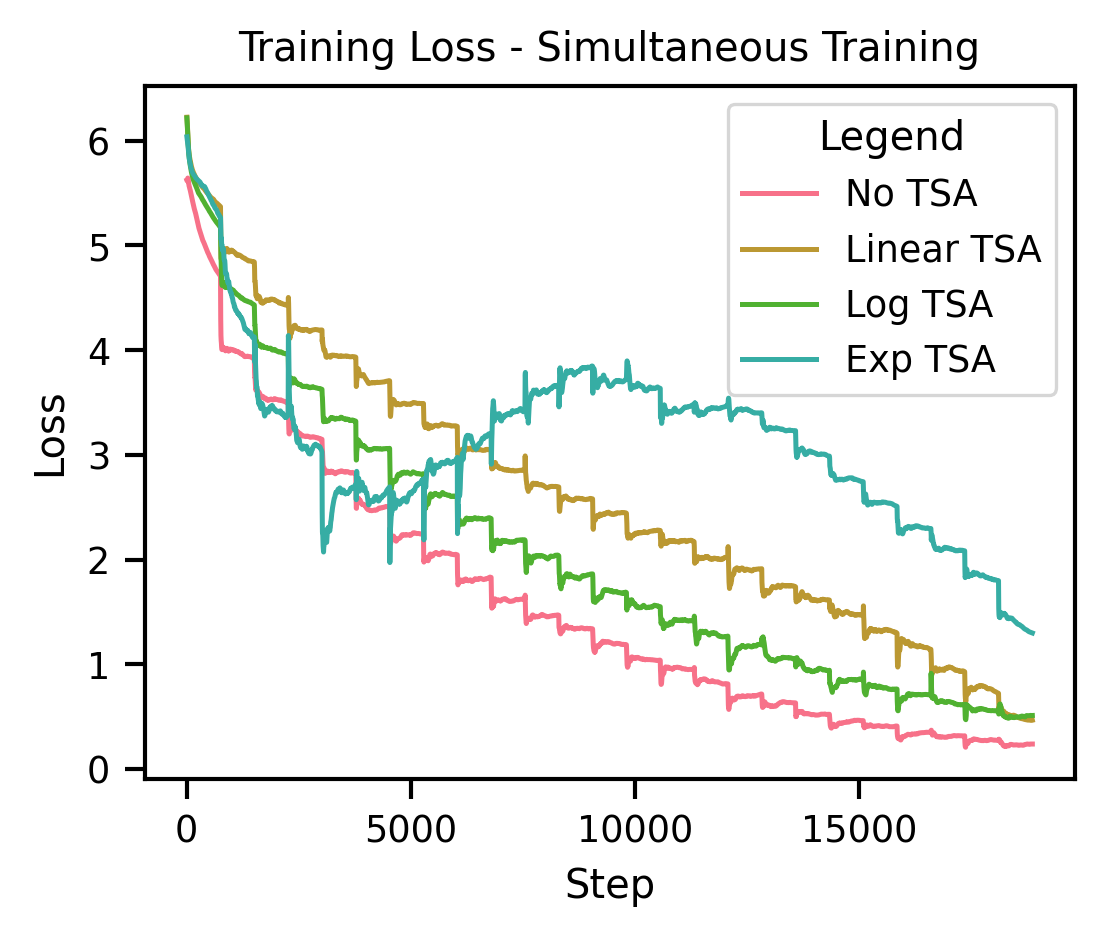
\includegraphics[height=5cm]{pics/tsa-simul-loss.png} }}%
  \caption{Comparing characteristics of different TSA threshold functions}%
  \label{fig:tsa}%
\end{figure}

\subsubsection{Various Advanced Data Augmentation}
\label{sec:var_data_aug}
% about the quality of them prediciting alone; and used with training dataset
We explored three distinct data augmentation techniques: back-translation, 
random-mask completion, and sentence completion. The model was trained using the 
augmented training data, while preserving the original labels for the supervised task. 
This approach allowed us to evaluate the quality of the data augmentation, as detailed 
in Appendix Table \ref{tab:data_aug_comp}.

Back-translation performed as anticipated, matching the original model's performance. 
Random-mask completion underperformed likely due to factual alterations during the fill-in-the-blank 
process. Unexpectedly, sentence completion also fell short, potentially due to training 
exclusively on PLM-summarized data and then inferring from original text. For instance, in the 
STS task, a sentence pair like "A man plays the guitar and sings." and "A man is singing and 
playing a guitar." with a similarity of 5.0, was simplified by sentence completion to "He is a 
musician." for both sentences. This simplification poses challenges when the model infers from 
original text data.

\subsubsection{Training in SSL settings}
% Please add the following required packages to your document preamble:
% \usepackage{booktabs}
We henceforth refer to the fine-tuned BERT model, which employs the Fused Sentence 
Embedding technique and the simultaneous 
training strategy discussed in section \ref{sec:baseline_ext}, 
as our baseline extension model. We now explore how SSL settings 
can enhance supervised learning outcomes.

\begin{table}[htbp]
  \centering
  \caption{Comparisons of Dev model performance in SSL settings}
  \label{tab:ssl_res}
  \begin{tabular}{@{}lcccc@{}}
    \toprule
    \textbf{Model}                               & \textbf{SST5}  & \textbf{QQP}   & \textbf{STS}   & \textbf{Avg. Accuracy} \\ \midrule
    Baseline Extension                           & 0.501          & 0.829          & 0.852          & 0.752                  \\
    BE + Linear TSA                              & 0.520          & \textbf{0.836} & 0.861          & \textbf{0.762}         \\
    BE + Linear TSA + UDA Back Translation       & \textbf{0.520} & 0.821          & \textbf{0.862} & 0.758                  \\
    BE + Linear TSA + UDA Sentence Completion    & 0.506          & 0.820          & 0.853          & 0.751                  \\
    BE + Linear TSA + UDA Random-mask Completion & 0.520          & 0.808          & 0.827          & 0.747                  \\ \bottomrule
    \end{tabular}
\end{table}

As shown in Table \ref{tab:ssl_res}, Linear TSA enhances the baseline extension model 
across tasks by focusing more on challenging examples rather than overfitting on simpler ones. 
However, training on the full dataset with data augmentation as a regularization term does 
not further boost the model's performance.
While UDA offers slight improvements on SST5 and STS, it underperforms on the QQP task. This 
shortcoming may stem from ineffective prompting to the LLaMA-3 Chat (8B) model. We observed 
that many back-translation responses closely mirror the unlabeled data. 
Although prompting through the chain-of-thought technique, LLaMA-3 Chat (8B) appears to 
increasingly depend on input sentences, often producing identical back-translations. 
This redundancy undermines UDA's effectiveness, as the KL-divergence loss becomes zero, 
potentially increasing noise in the gradient updates.

Another potential factor is our use of trained datasets to generate "unlabeled" datasets, 
rather than incorporating new samples outside of the training distribution. This absence 
of fresh samples may limit UDA's effectiveness in improving the model's generalization.




\subsection{Results}
% Report the quantitative results that you have found. Use a table or plot to compare results and compare against baselines.
% \begin{itemize}
%     \item If you're a default project team, you should \textbf{report the accuracy and Pearson correlation scores you obtained on the test leaderboard} in this section. You can also report dev set results if you'd like. 
%     \item Comment on your quantitative results. Are they what you expected? Better than you expected? Worse than you expected? Why do you think that is? What does that tell you about your approach?
% \end{itemize}
% Please add the following required packages to your document preamble:
% \usepackage{booktabs}
We now discuss our model's performance on the Dev and Test sets. Our final model integrates 
the baseline extension with linear TSA (BE + Linear TSA in Table \ref{tab:ssl_res}).
The results in Table \ref{tab:final_res} demonstrate that TSA effectively mitigates 
overfitting, yielding consistent performance across both the Dev and Test sets.

\begin{table}[htbp]
  \centering
  \caption{Final model performance on both Dev and Test set}
  \label{tab:final_res}
  \begin{tabular}{@{}lcccc@{}}
  \toprule
           & \textbf{SST5}  & \textbf{QQP}   & \textbf{STS}   & \textbf{Avg. Accuracy} \\ \midrule
  Dev Set  & \textbf{0.520} & 0.836          & 0.861          & 0.762                  \\
  Test Set & 0.517          & \textbf{0.839} & \textbf{0.866} & \textbf{0.763}         \\ \bottomrule
  \end{tabular}
\end{table}


\section{Analysis}
% Your report should include \textit{qualitative evaluation}. That is, try to understand your system (e.g., how it works, when it succeeds and when it fails) by inspecting key characteristics or outputs of your model.

To gain a deeper understanding of the model's performance, we carried out both quantitative and 
qualitative analyses across the three tasks. In essence, the model exhibits a strong grasp of 
sentiment analysis and sentence-pair similarity analysis. However, it has challenges with the inherent 
ambiguities in human-annotated data, the differentiation of sentence roles, and the discernment 
of subtle sentiment variations when sentences employ identical or similar words.

\begin{figure}[H]%
  \centering
  \subfloat[SST5 Dev Set Confusion Matrix normalized to predicted labels]
  {{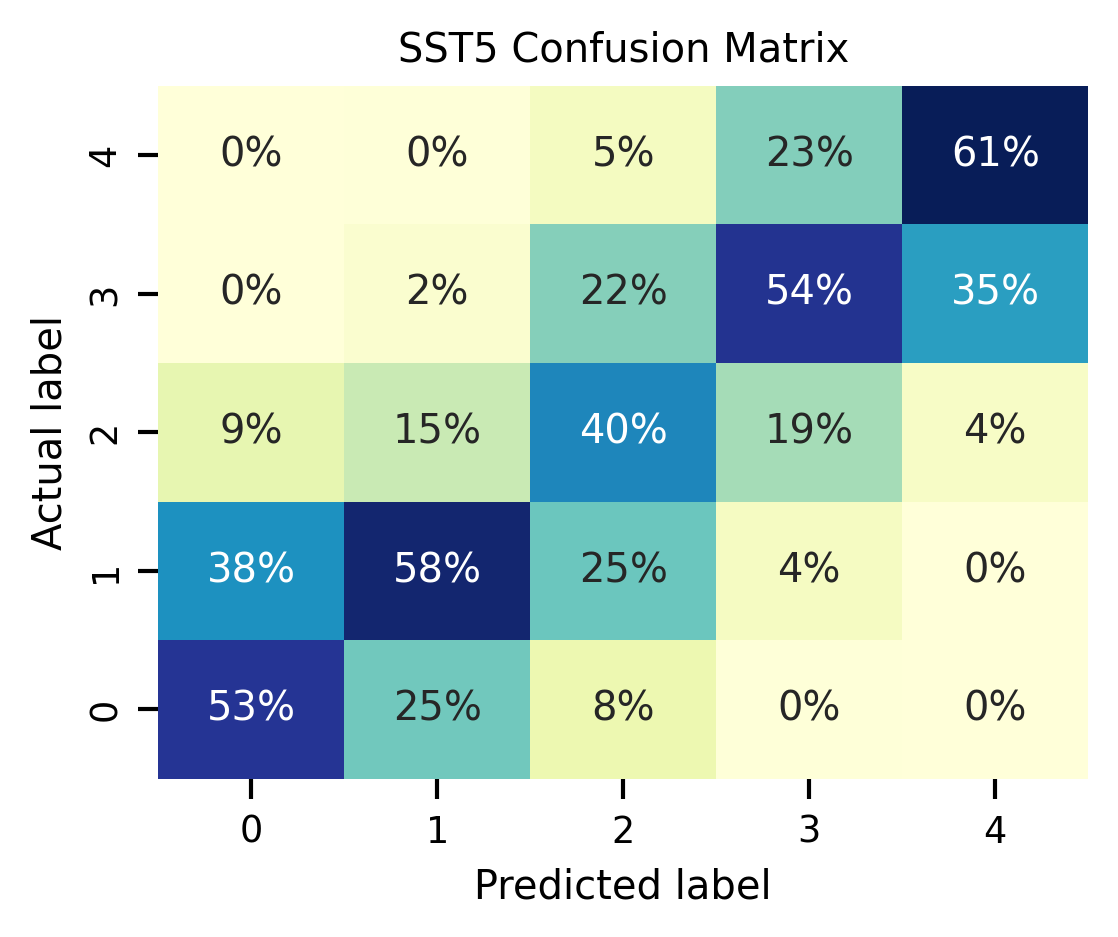
\includegraphics[width=0.3\textwidth]{pics/sst5.png} }}%
  \hfill
  \subfloat[QQP Dev Set Confusion Matrix normalized to predicted labels]
  {{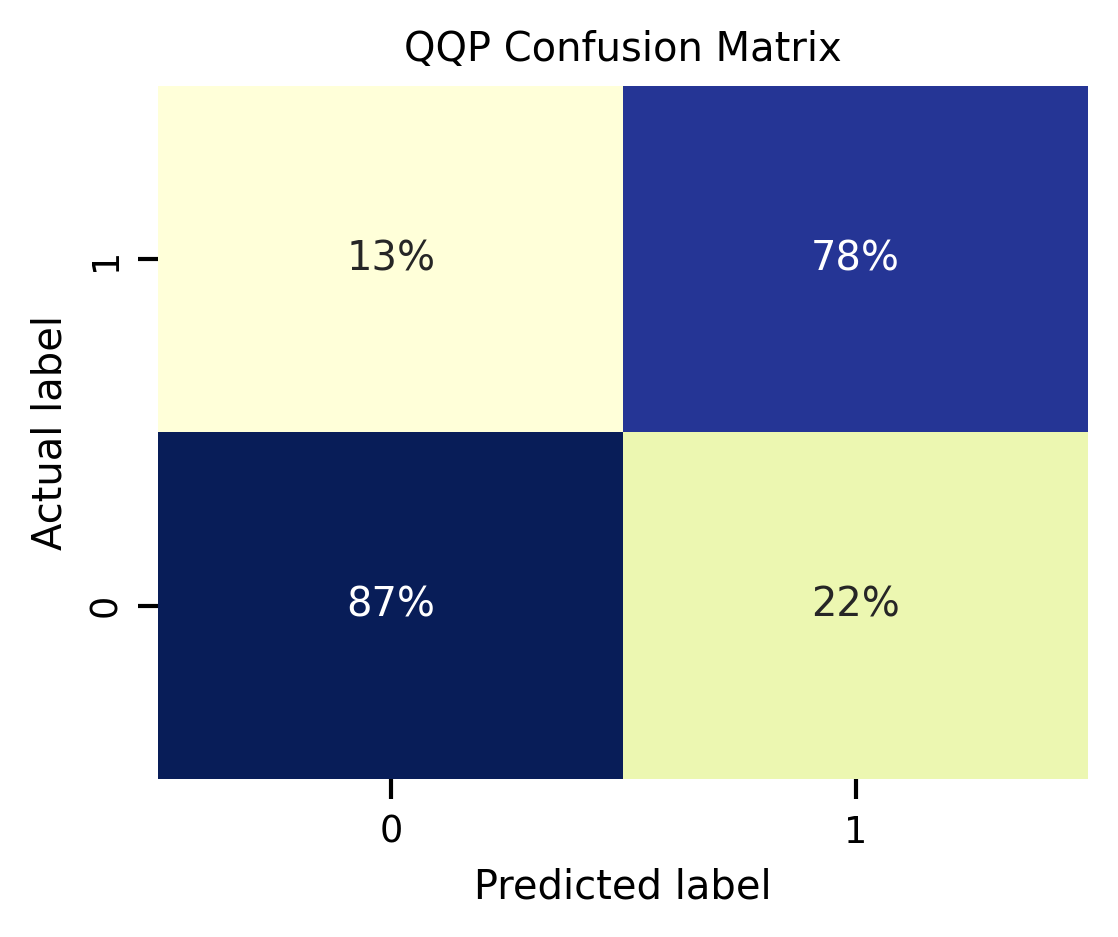
\includegraphics[width=0.3\textwidth]{pics/qqp.png} }}%
  \hfill
  \subfloat[STS Correlation Plot, line showing best fit]
  {{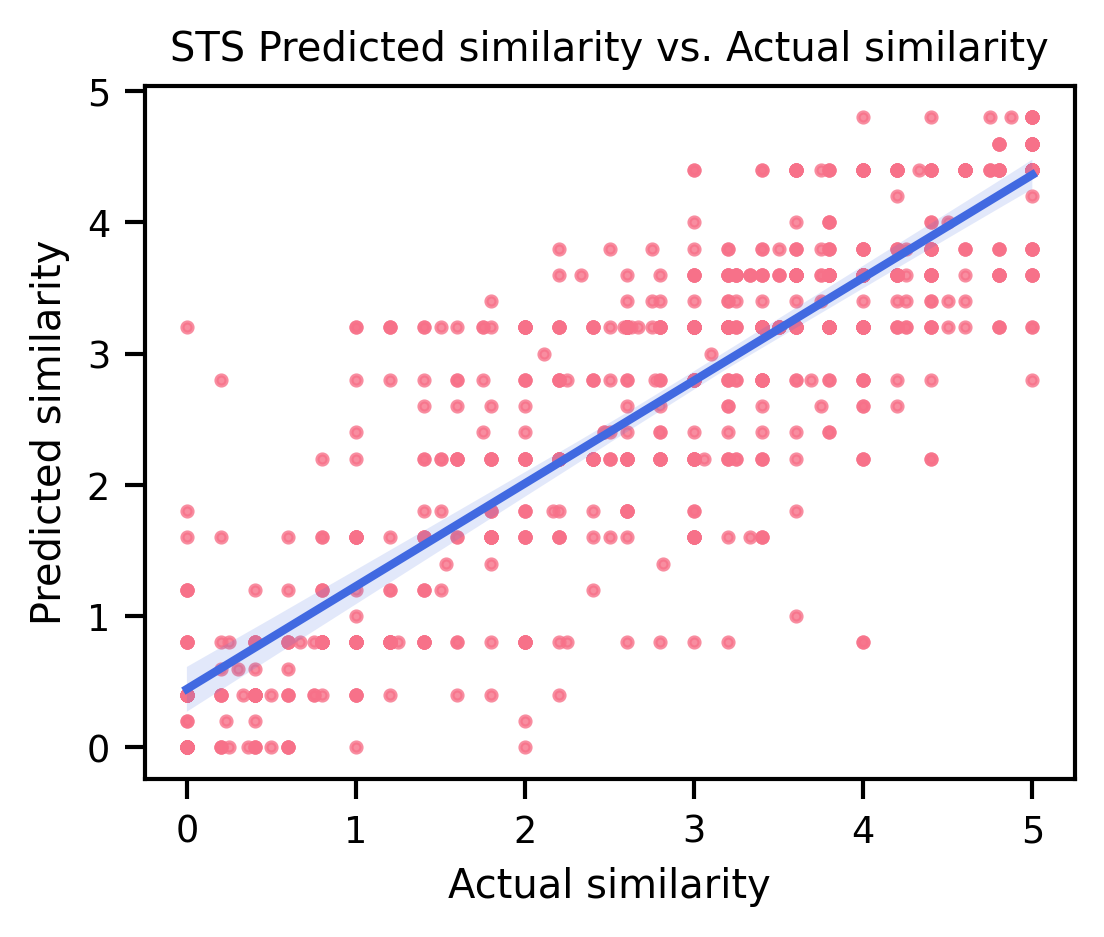
\includegraphics[width=0.3\textwidth]{pics/sts.png} }}%
  \caption{Analysis of Dev set performance of the model
  }%
  \label{fig:analysis}%
\end{figure}

\textbf{Fine-grained Sentiment Analysis SST5} As shown in Figure \ref{fig:analysis}(a), 
the model demonstrates a robust understanding of sentiment. Misclassifications primarily 
occur between adjacent categories. Despite not explicitly training the SST5 task using an 
ordinal categorical approach, the model effectively learns and interprets sentiment. 
Interestingly, the model performs better on extreme sentiments than neutral ones. This 
performance discrepancy may be due to inherent ambiguities in the text and biases from human 
evaluators. For instance, the sentence "Hilariously inept and ridiculous." was labeled as 
somewhat positive. However, both our model and ChatGPT-4 assign it a 
somewhat negative rating. Absent further context, the sentiment of this sentence remains 
open to interpretation.

\textbf{Paraphrase Detection QQP} As illustrated in Figure \ref{fig:analysis}(b), the model 
exhibits lower precision in the positive class compared to the negative class. Two primary 
themes emerge from the cases incorrectly classified as positive: The first involves sentences 
with identical or similar words but in different orders, such as the pair "Can MIT PhD students 
have a Harvard PhD adviser?" and "Can Harvard PhD students have an MIT PhD adviser?". The model 
struggles to distinguish the respective roles in each sentence, suggesting potential areas for 
improvement such as incorporating dependency or POS tags and advanced positional embeddings into 
the model setup. The second theme pertains to ambiguities in human-labeled data. For instance, 
the pair "Why did you deactivate your Facebook account?" and "What are the benefits of 
deactivating your Facebook account?" is labeled as non-paraphrase. However, one could interpret 
these sentences as having the same intent, thus considering them as paraphrases.

\textbf{Textual Similarity STS} Similar to the SST5 task, the model is trained in a multi-class
manner, capturing the relative relationship between numerical classes without requiring
additional ordinal categorical training. Misclassifications are typically found around
the adjacent areas of the true score. As observed in Figure \ref{fig:analysis}(c), the fitted 
prediction line has a slope less than 1, indicating the model produces a narrower range
of scores compared to actual human labels. This may be attributed to the model's tendency not to 
assign extreme scores when sentences share common words. For instance, the sentences "Work into 
it slowly." and "It seems to work." were judged by humans to have 0.0 similarity, yet the model 
assigns a 3.2 score, given that 50\% of the words are identical. This 
highlights the model's difficulty in capturing sentiment 
nuances when sentences use the same words.


	

\section{Conclusion}
% Summarize the main findings of your project and what you have learned. Highlight your achievements, and note the primary limitations of your work. If you'd like, you can describe avenues for future work.
In this study, we effectively enhanced BERT\textsubscript{BASE} embeddings' performance across 
various NLP tasks using a multitask learning strategy and incorporating semi-supervised learning 
techniques. Our experiments revealed that the fused sentence embedding approach and simultaneous 
training schedule significantly boosted the model's performance in all downstream tasks. 
Moreover, the integration of the UDA framework, particularly the TSA component, further 
amplified our model's capabilities, despite the limitations in the quality of data augmentation. 
These findings underscore the potential of advanced PLMs in SSL settings and the importance of 
high-quality data augmentation for the success of this framework. Future research could focus 
on exploring more efficient data augmentation approaches, training paradigms, and advanced 
language features to overcome existing challenges and build more robust and 
generalizable NLP models.

\section{Ethics Statement}
% What are the ethical challenges and possible societal risks of your project, and
% what are mitigation strategies?
The integration of BERT with UDA in semi-supervised NLP tasks introduces societal and ethical  
concerns. While fine-tuning BERT with UDA can reduce human labeling costs, it may escalate 
computational expenses due to generation of augmented datasets for large amount of 
unsupervised datasets via PLM prompts,
which could have a significant environmental impact when implemented at scale.
Recent progress in few-shot and zero-shot learning with advanced PLMs 
(\cite{meng2022generating,wang2021zerolabel}) suggests training paradigms that are more 
efficient than UDA, potentially leading to more streamlined inference.

On the other hand, bias and toxicity amplification might present in the process of 
data augmentation via PLM prompts. 
Existing biases or toxic language 
in training data and PLMs can be exacerbated in semi-supervised training setups during the 
generation of augmented datasets. Several strategies have been proposed to address these issues 
in PLMs. For instance, \cite{ma-etal-2020-powertransformer} introduced PowerTransformer, which 
minimizes biases in text and paraphrases. Employing existing models or APIs to scrutinize PLM-generated data can aid in filtering out 
biased and toxic content and rephrasing biased text, thereby mitigating the amplification issue.



\newpage
\bibliographystyle{acl_natbib}
\bibliography{references}

\newpage
\appendix
\renewcommand{\thefigure}{A\arabic{figure}}
\renewcommand{\thetable}{A\arabic{table}}
\setcounter{figure}{0}
\setcounter{table}{0}

\section{Appendix}
% If you wish, you can include an appendix, which should be part of the main PDF, and does not count towards the 6-8 page limit.
% Appendices can be useful to supply extra details, examples, figures, results, visualizations, etc. that you couldn't fit into the main paper. However, your grader \textit{does not} have to read your appendix, and you should assume that you will be graded based on the content of the main part of your paper only.
\subsection{Training strategies}
\label{sec:appdx_train_strategy}
Simultaneous training consistently outperforms sequential training in producing 
multitask models, as evidenced by the results in Table \ref{tab:baseline_ext} 
and Appendix Table \ref{tab:baseline_ext_seq}. 
Simultaneous training benefits from less frequent model updates, occurring only a third 
as often as in sequential training when trained for an equal number of epochs (updating
once per three tasks versus updating once per task in sequential training). 
Each step averages the loss from the three tasks, yielding an averaged gradient that
stabilizes parameter updates.

In contrast, sequential training has more frequent model 
updates, potentially introducing noise into the gradient updates. Furthermore, during 
sequential training, the three tasks are processed in chunks, meaning the model updates 
gradients based on a single task's data before moving on to the next. If the tasks are 
not well synergized, as indicated by the weak correlation of the SST5 task with the QQP 
and STS tasks in Table \ref{tab:baseline_ext}, this could create conflicting gradient 
descent directions and introduce additional noise, thereby negatively impacting model 
performance.

\begin{table}[htbp]
  \centering
  \caption{Comparisons of Baselines and Extensions on Dev Data, training three tasks sequentially}
  \label{tab:baseline_ext_seq}
  \begin{tabular}{@{}lcccc@{}}
    \toprule
    \textbf{Model}                & \textbf{SST5}  & \textbf{QQP}   & \textbf{STS}   & \textbf{\begin{tabular}[c]{@{}c@{}}Avg. Accuracy\end{tabular}} \\ \midrule
    Baseline (last-layer only)    & 0.309          & 0.667          & 0.209          & 0.527                                                             \\
    Arc1-Simple Concat            & 0.476          & 0.732          & 0.363          & 0.630                                                             \\
    Arc1-Absolute difference      & \textbf{0.509} & 0.712          & 0.530          & 0.662                                                             \\
    Arc1-Cosine Similarity        & 0.486          & 0.503          & 0.495          & 0.579                                                             \\
    Arc1-Dot Product Attention    & 0.473          & 0.728          & 0.420          & 0.637                                                             \\
    Arc2-Fused Sentence Embedding & 0.486          & \textbf{0.823} & \textbf{0.832} & \textbf{0.742}                                                    \\ \bottomrule
    \end{tabular}
\end{table}

\subsection{Various data augmentation}

We trained the model using the augmented dataset, while preserving the original labels 
for the supervised task. Back-translation performed comparably to training with real text. 
However, the other approaches did not prove suitable for standalone use.

\begin{table}[htbp]
  \centering
  \caption{Training on full augmented dataset as supervised learning}
  \label{tab:data_aug_comp}
  \begin{tabular}{@{}lcccc@{}}
  \toprule
  \textbf{Augmentation Approach} & \textbf{SST5} & \textbf{QQP} & \textbf{STS} & \textbf{Avg. Accuracy} \\ \midrule
  Back Translation               & 0.510         & 0.826        & 0.802        & 0.746                  \\
  Random Mask Completion         & 0.470         & 0.781        & 0.723        & 0.704                  \\
  Sentence Completion            & 0.411         & 0.728        & 0.630        & 0.651                  \\ \bottomrule
  \end{tabular}
\end{table}

\end{document}